\section{Date: 2026-10-04}
\noindent \textbf{Series ID: CMTNURN} 

\noindent This series is titled Unemployment Rate in Mountain Census Division and has a frequency of Monthly. The units are Percent and the seasonal adjustment is Not Seasonally Adjusted.The observation start date is 1976-01-01 and the observation end date is 2026-08-01.The popularity of this series is 1. \\ 

\noindent \textbf{Series ID: SWSTPCEGAS} 

\noindent This series is titled Personal Consumption Expenditures: Nondurable Goods: Gasoline and Other Energy Goods for Southwest BEA Region and has a frequency of Annual. The units are Millions of Dollars and the seasonal adjustment is Not Seasonally Adjusted.The observation start date is 1997-01-01 and the observation end date is 2025-01-01.The popularity of this series is 1. \\ 

\subsection{Raw Regression}
\noindent Regresses the two series against each other directly. A significant result here can come just as easily from both series sharing a long-run trend as from any real relationship.

\begin{center}
\begin{tabular}{lclc}
\toprule
\textbf{Dep. Variable:}       & value\_fred\_SWSTPCEGAS & \textbf{  R-squared:         } &     0.010   \\
\textbf{Model:}               &           OLS           & \textbf{  Adj. R-squared:    } &    -0.027   \\
\textbf{Method:}              &      Least Squares      & \textbf{  F-statistic:       } &    0.2701   \\
\textbf{Date:}                &     Sun, 04 Oct 2026    & \textbf{  Prob (F-statistic):} &    0.608    \\
\textbf{Time:}                &         16:03:27        & \textbf{  Log-Likelihood:    } &   -321.57   \\
\textbf{No. Observations:}    &              29         & \textbf{  AIC:               } &     647.1   \\
\textbf{Df Residuals:}        &              27         & \textbf{  BIC:               } &     649.9   \\
\textbf{Df Model:}            &               1         & \textbf{                     } &             \\
\textbf{Covariance Type:}     &        nonrobust        & \textbf{                     } &             \\
\bottomrule
\end{tabular}
\begin{tabular}{lcccccc}
                              & \textbf{coef} & \textbf{std err} & \textbf{t} & \textbf{P$> |$t$|$} & \textbf{[0.025} & \textbf{0.975]}  \\
\midrule
\textbf{const}                &    3.732e+04  &     9995.746     &     3.734  &         0.001        &     1.68e+04    &     5.78e+04     \\
\textbf{value\_fred\_CMTNURN} &     894.4909  &     1721.253     &     0.520  &         0.608        &    -2637.229    &     4426.211     \\
\bottomrule
\end{tabular}
\begin{tabular}{lclc}
\textbf{Omnibus:}       &  1.615 & \textbf{  Durbin-Watson:     } &    0.254  \\
\textbf{Prob(Omnibus):} &  0.446 & \textbf{  Jarque-Bera (JB):  } &    1.026  \\
\textbf{Skew:}          & -0.061 & \textbf{  Prob(JB):          } &    0.599  \\
\textbf{Kurtosis:}      &  2.087 & \textbf{  Cond. No.          } &     19.6  \\
\bottomrule
\end{tabular}
%\caption{OLS Regression Results}
\end{center}

Notes: \newline
 [1] Standard Errors assume that the covariance matrix of the errors is correctly specified.

\begin{figure}
\centering
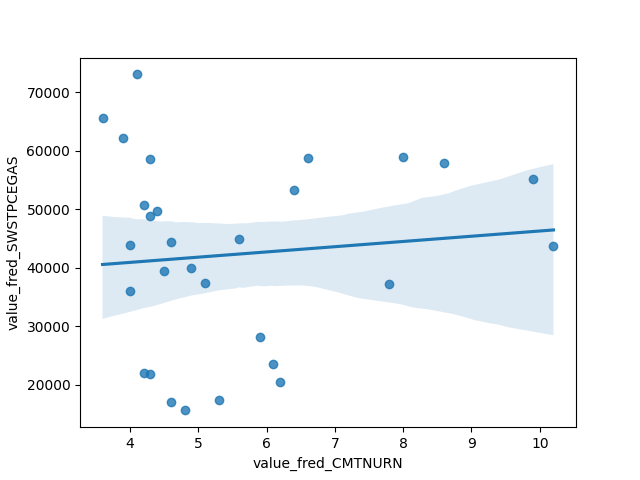
\includegraphics[scale = 0.9]{plots/plot_2026-10-04.png}
\caption{Raw Regression Plot for 2026-10-04}
\end{figure}
\newpage
\subsection{Detrended Regression}
\noindent Regresses the residuals of each series after removing its own linear time trend, so a shared trend can no longer drive the result on its own. A relationship that stays significant here is better evidence of a genuine link between the two series.

\begin{center}
\begin{tabular}{lclc}
\toprule
\textbf{Dep. Variable:}                  & value\_fred\_SWSTPCEGAS\_detrended & \textbf{  R-squared:         } &     0.151   \\
\textbf{Model:}                          &                OLS                 & \textbf{  Adj. R-squared:    } &     0.120   \\
\textbf{Method:}                         &           Least Squares            & \textbf{  F-statistic:       } &     4.809   \\
\textbf{Date:}                           &          Sun, 04 Oct 2026          & \textbf{  Prob (F-statistic):} &   0.0371    \\
\textbf{Time:}                           &              16:03:28              & \textbf{  Log-Likelihood:    } &   -300.91   \\
\textbf{No. Observations:}               &                   29               & \textbf{  AIC:               } &     605.8   \\
\textbf{Df Residuals:}                   &                   27               & \textbf{  BIC:               } &     608.5   \\
\textbf{Df Model:}                       &                    1               & \textbf{                     } &             \\
\textbf{Covariance Type:}                &             nonrobust              & \textbf{                     } &             \\
\bottomrule
\end{tabular}
\begin{tabular}{lcccccc}
                                         & \textbf{coef} & \textbf{std err} & \textbf{t} & \textbf{P$> |$t$|$} & \textbf{[0.025} & \textbf{0.975]}  \\
\midrule
\textbf{const}                           &   -8.162e-10  &     1494.086     & -5.46e-13  &         1.000        &    -3065.611    &     3065.611     \\
\textbf{value\_fred\_CMTNURN\_detrended} &    1865.7194  &      850.795     &     2.193  &         0.037        &      120.033    &     3611.406     \\
\bottomrule
\end{tabular}
\begin{tabular}{lclc}
\textbf{Omnibus:}       &  0.152 & \textbf{  Durbin-Watson:     } &    1.116  \\
\textbf{Prob(Omnibus):} &  0.927 & \textbf{  Jarque-Bera (JB):  } &    0.308  \\
\textbf{Skew:}          &  0.143 & \textbf{  Prob(JB):          } &    0.857  \\
\textbf{Kurtosis:}      &  2.583 & \textbf{  Cond. No.          } &     1.76  \\
\bottomrule
\end{tabular}
%\caption{OLS Regression Results}
\end{center}

Notes: \newline
 [1] Standard Errors assume that the covariance matrix of the errors is correctly specified.

\begin{figure}
\centering
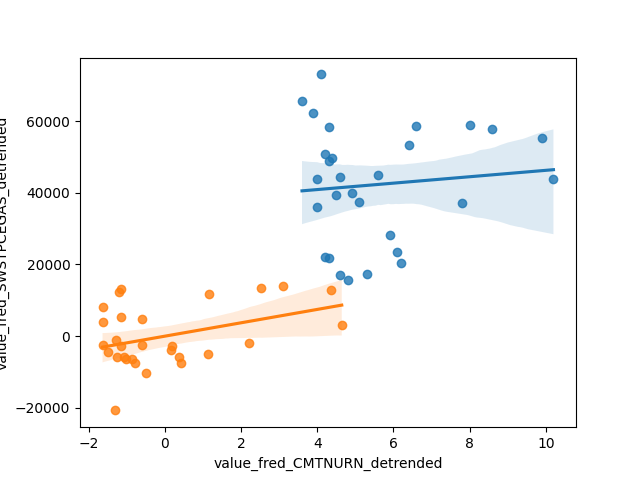
\includegraphics[scale = 0.9]{plots/plot_2026-10-04_detrended.png}
\caption{Detrended Regression Plot for 2026-10-04}
\end{figure}
\newpage
